\section{Literature Review}

\subsection{History of Food Waste}

\enquote*{Food waste is especially visible when its prevention is being counselled.}~\cite{evans_brief_2012}
Cookery books dating back to the mid-19th century reference the need to properly manage food once brought
into the house.~\cite{beeton_mrs_1907} Such notions continued until the 1950s where significant shifts
occurred following the end of post World War II rationing attributed to the success of policies intended
to restore the production of farmers and leading to a global food surplus.~\cite{evans_brief_2012}

This prolonged period of surplus is believed to have led to an ideology of \enquote*{technological optimism},
where it was believed that technology would solve all problems including food waste~\cite{krier_-easy_1985} and
therefore avoiding waste was no longer a concern.

\subsection{Current State of Food Waste and its Impacts}

Following the 2008 financial crisis, food prices have continued to increase leading to elevated consumer concern
as cheap food could no longer be taken for granted~\cite{evans_brief_2012} which has been further worsened by the
ongoing war in Ukraine.~\cite{ben_hassen_impacts_2022}

As of 2013, 4.4 million tons of avoidable food waste was generated in the UK,~\cite{quested_spaghetti_2013} the
reduction of which could have \enquote*{a substantial positive environmental effect}.~\cite{quested_spaghetti_2013}
In that same. While more producers are taking steps to reduce waste, this only accounts for ~20\% of all large producers
as of 2022.~\cite{wrap_food_2023} Factors found to reduce food waste include planning meals in advance and checking
levels of food before shopping.~\cite{quested_spaghetti_2013}

Presently, much of the food waste generated is disposed of in landfills~\cite{iacovidou_food_2012}, which produces
methane, a greenhouse gas 28 times as potent as carbon dioxide,~\cite{marmier_methane_2020} and results in higher
environmental impacts than other methods of disposal even if the majority of the methane is captured and utilized,
being the only disposal option that resuts in a net increase of emissions compared to consumption.~\cite{moult_greenhouse_2018}

\subsection{Prior Work in Subject Area}
\subsubsection{Food Waste}
Stefan et al.\ found that \enquote*{the intention not to waste food does not have a
significant effect on reported food waste}. Instead, planning before shopping to
check what is already available was found to lead to a reduction in food waste.~\cite{stefan_avoiding_2013}

As planning before shopping is a key factor in reducing food waste, the need for a system
that tracks how much of each ingredient is available was identified. This would allow for
users to know plan meals based on what they already have, reducing the need to buy more ingredients
and thus reducing food waste.

\subsubsection{Meal Planning}
\label{sec:overload_intro}While providing a user with variety of choices can improve their satisfaction
with the overall system, care must be taken to avoid information overload.
Bollen et al.\ found that offering a more limited set items predicted to be among a user's
highest rated, followed by a larger set of more varied items with lower rankings, led to
higher satisfaction on average.~\cite{bollen_understanding_2010}

\subsubsection{Techniques Common to Food Reccomender Systems}
There exist a broad range of techniques used by food recommendation systems, using both machine learning
and statistical models, the most popular method in existing studies being machine learning based on the
contents of recipes. Most of which were not personalized to the individual user.~\cite{bondevik_systematic_2024}

Among prior systems, the majority source their training data from textual data with the most commonly used
attributes being ingredients, cooking instructions, and the recipe title itself. There has been limited research
into combining multiple attributes of the recipe or giving attributes different weights.~\cite{chen_cross-modal_2017} These factors are often
considered to be merely a subject for future research or unimportant, which is believed to degrade the performance
of systems.~\cite{bondevik_systematic_2024}

\subsection{Recipe Name-based Suggestions}\label{sec:recipe_name_suggestions}

One method of evaluating the similarity of recipes is to compare their names which is considered to
give similar results to human judgement.~\cite{trattner_learning_2020,starke_serving_2021} This method
combined with a sentence embedding model was selected for the \chef{} app.

There are many determining factors behind the food choices and preferences of people~\cite{leng_determinants_2017,franchi_food_2012}
giving credit to recommendation systems that incorporate multiple factors. However, prior studies have
found recipe names to be important in the decision-making process as descriptive names are more likely to be
selected.~\cite{ohlhausen_when_2020} For this reason, the \chef{} app will use recipe names in its measure of similarity.

\subsubsection{Effectiveness Outside of Western Cuisine}
While western recipe names are typically constructed in a predictable format
that indicates what kind of recipe it is, this is not the case world-wide.
For example, Chinese recipe names often bear little resemblance to the contents
of the recipe itself.~\cite{wang_substructure_2008} This limits the effectiveness
of suggestions systems based on names and as such a more complex system as discussed
by Wang et al.\ would be needed.

\subsection{The Research Questions}

The motivation for the \chef{} app is two-fold: to reduce the environmental impact of food waste and to
save costs for households by allowing them to collectively track what ingredients are available to them.
This shall be achieved through implementing a system meeting the following goals:

The goals of the \chef{} app are to provide a robust system that allows for users to track what ingredients they have in a
convenient manner, and to suggest recipes based on these ingredients, user preferences, dietary requirements, and to find
similar recipes that meet these criteria.

An additional goal is to evaluate how effectively similar recipes can be categorized based on their titles
and a sentence embedding model. This will be done by comparing the results of the model to a human judgement
of whether the suggested recipes are similar or not.

Finally, the recipe similarity model will be tested to see if it can also categorize recipes into meal types
based on the same criteria. This will again be evaluated against human judgement on whether the categorization
is correct and how often it is correct.

\section{Competitor Analysis}\label{sec:competitor_analysis}

As part of the development of \chef{}, a competitor analysis has been performed on several existing solutions as part of research
into the problem domain. These solutions, while useful, had limitations as discussed below. The \chef{} app aims to address
these limitations and provide a more useful solution. The full list of competitors analysed is provided in Section~\ref{sec:competitors}.

SuperCook and MyFridgeFood both include feature an account system
that saves a user's list of available ingredients. Creating an account also allows for recipes to be favourited/bookmarked
which would then be shown on a dedicated page. SuperCook additionally shows which of the user's favourite recipes
can be made using available ingredients and which ingredients are missing. Both apps also use exclusively imperial
units for ingredients that are not understood by the majority of the world. The \chef{} app will use metric units by default
as it is targeted at a UK audience.

However, neither of these apps has a system for sharing ingredient lists between users or specifying disliked ingredients. These features would be useful for households with multiple people.
Additionally, the only way to update available ingredients is to manually add or remove them which is time-consuming and tedious. There is no tracking for the quantity of
each ingredient, so there is no way to know if the user has enough of an ingredient without checking manually.

Neither app tracks which recipes have been made recently, so there is no way to avoid suggesting similar recipes to ones that have been recently made which could lead to
users getting bored with eating the same meals over and over.

MyFridgeFood has a feature to submit new recipes which are shared between all users. This is a useful feature as it allows for the community to contribute to the database
of recipes, however, these cannot be kept private to just one user.

\subsection{User Reviews}

A frequent complaint about MyFridgeFood was that it suggested
recipes that users lacked ingredients for. See figure~\ref{rev:review_missing_ingredients} for an example.

A different user found that MyFridgeFood gave them suggestions that were too similar to each
other. See figure~\ref{rev:review_lack_variety} for the review.

\section{Product Requirements}

\todo{Where did these specificvations come from? How did you develop them?}

% https://tex.stackexchange.com/questions/503668/increment-a-counter
\newcounter{functionalreqcounter}
\newcommand{\requirementtype}{FR}
% Usage:
%   #1 Requirement
%   #2 Source
%   #3 Priority
%   #4 Implemented (yes/no)
\newcommand{\requirement}[4]{%
    \requirementtype\stepcounter{functionalreqcounter}\arabic{functionalreqcounter}%
    % Don't have much space to work with, so flushright looks messy.
    &\raggedright#1&#2&#3&#4\\}

\begin{longtable}{lp{128pt}lll}
    \caption{Functional Requirements}\label{tab:functional_requirements}
    \\\toprule
    \textbf{ID} & \textbf{Requirement} & \textbf{Source} & \textbf{Priority} & \textbf{Implemented} \\\midrule

    \requirement{\label{req:web_app}\newcounter{webappid}\setcounter{webappid}{\thefunctionalreqcounter}%
        \textbf{Web app.} The system \textbf{must} be a web app that fetches from a REST API}
    {Competitor Analysis}
    {Must-have}
    {Yes}

    \requirement{\textbf{User registration.} The system \textbf{must} allow users to sign up and log in to the app.}
    {Competitor Analysis}
    {Must-have}
    {Yes}

    \requirement{\textbf{Share ingredient lists.} The system \textbf{must} allow for multiple users to share one \virtualfridge{}}
    {Competitor Analysis}
    {Must-have}
    {Partially}

    \requirement{\textbf{Select dietary requirements/preferences.} The system \textbf{must} \newline
        allow for users to select their dietary requirements and preferences, such as allergies or disliked ingredients.}
    {Competitor Analysis}
    {Must-have}
    {Yes}

    \requirement{\label{req:suggestion}\newcounter{suggestionid}\setcounter{suggestionid}{\thefunctionalreqcounter}%
        \textbf{Recipe Suggestion.} The system \textbf{must} suggest recipes based on the user's available ingredients}
    {Competitor Analysis}
    {Must-have}
    {Yes}

    \requirement{\label{req:overload}\newcounter{overloadid}\setcounter{overloadid}{\thefunctionalreqcounter}%
        \textbf{Prevent Choice Overload.} The system \textbf{could} include measures to prevent choice overload.}
    {Literature review}
    {Could-have}
    {Experimental}

    \requirement{\textbf{Avoid recipes with missing ingredients.} The system \textbf{must} not suggest recipes that the user
    is missing ingredients for unless explicitly requested.}
    {Competitor Analysis}
    {Must-have}
    {Yes}

    \requirement{\label{req:sources}\newcounter{sourcesid}\setcounter{sourcesid}{\thefunctionalreqcounter}%
    \textbf{Include sources.} The system \textbf{must} include its sources for recipes.}
    {Trivial}
    {Must-have}
    {Yes}

    \requirement{\label{req:manual_add}\newcounter{manualaddid}\setcounter{manualaddid}{\thefunctionalreqcounter}%
        \textbf{Manually add ingredients.} The system \textbf{must} allow users to manually add ingredients to their \virtualfridge}
    {Competitor Analysis}
    {Must-have}
    {Yes}

    \requirement{\label{req:data_flexible}\newcounter{flexibleid}\setcounter{flexibleid}{\thefunctionalreqcounter}%
    \textbf{Flexible Data Sources.} The system \textbf{should} be flexible regarding the dataset it uses}
    {Dataset Selection}
    {Should-have}
    {Yes}

    \requirement{\label{req:scan_barcode}\newcounter{scanbarcodeid}\setcounter{scanbarcodeid}{\thefunctionalreqcounter}%
        \textbf{Scan barcodes.} The system \textbf{should} allow the user to scan the barcodes of ingredients to add
    them to their \virtualfridge}
    {Use Case Analysis}
    {Should-have}
    {Yes}

    \requirement{\label{req:track_amounts}\newcounter{trackamountsid}\setcounter{trackamountsid}{\thefunctionalreqcounter}%
    \textbf{Track ingredient amounts.} The system \textbf{should} track the amount of each ingredient the user has available.}
    {Literature Review}
    {Should-have}
    {Yes}

    \requirement{\label{req:metric_units}\newcounter{metricunitsid}\setcounter{metricunitsid}{\thefunctionalreqcounter}%
        \textbf{Use metric units.} All units \textbf{should} be displayed in metric by default.}
    {Competitor Analysis}
    {Should-have}
    {Yes}

    \requirement{\label{req:imperial_units}\newcounter{imperialunitsid}\setcounter{imperialunitsid}{\thefunctionalreqcounter}%
        \textbf{Optionally use imperial units.} There \textbf{could} be an option to display imperial units instead of metric.}
    {Competitor Analysis}
    {Could-have}
    {No}

    \requirement{\label{req:scan_receipt}\newcounter{scanreceiptid}\setcounter{scanreceiptid}{\thefunctionalreqcounter}%
        \textbf{Scan receipt.} The system \textbf{could} allow the user to scan a receipt from a store to add ingredients
    to their \virtualfridge}
    {Use Case Analysis}
    {Could-have}
    {No}

    \requirement{\label{req:similar_recipes}\newcounter{findsimilarid}\setcounter{findsimilarid}{\thefunctionalreqcounter}%
    \textbf{Find similar recipes.} The system \textbf{should} use a machine learning model to find and suggest
    similar recipes to those that the user has previously made.}
    {Literature Review}
    {Should-have}
    {Yes}

    \requirement{\label{req:too_similar}\newcounter{toosimilarid}\setcounter{toosimilarid}{\thefunctionalreqcounter}%
    \textbf{Avoid repeating recipes.} The system \textbf{should} avoid suggesting recipes that are too similar
    to those that have been made recently using the same model as \hyperref[req:similar_recipes]{FR\arabic{findsimilarid}}}
    {Competitor Analysis}
    {Should-have}
    {No}

    \requirement{\label{req:meal_type}\newcounter{mealtypeid}\setcounter{mealtypeid}{\thefunctionalreqcounter}%
    \textbf{Predict meal types.} The system \textbf{should} predict the meal types of recipes.}
    {Use Case Analysis}
    {Should-have}
    {Partially}

    \requirement{\textbf{Single sign on.} The system \textbf{won't currently} support single sign on.}
    {Competitor Analysis}
    {Won't-have}
    {No}

    \requirement{\textbf{Add recipes.} The system \textbf{won't currently} allow for users to add their own recipes to the database.}
    {Competitor Analysis}
    {Won't-have}
    {No}

    \bottomrule
\end{longtable}

\setcounter{functionalreqcounter}{0}\renewcommand{\requirementtype}{NFR}
\begin{longtable}{lp{128pt}lll}
    \caption{Non-functional Requirements}\label{tab:non_functional_requirements}
    \\\toprule
    \textbf{ID} & \textbf{Requirement} & \textbf{Source} & \textbf{Priority} & \textbf{Implemented} \\\midrule

    \requirement{\textbf{Performance.} The system \textbf{should} be responsive to user input and requests to the API \textbf{should}
    be responded to in under 200ms on average.}
    {Trivial}
    {Should-have}
    {Yes}

    \requirement{\textbf{Reliability.} The system \textbf{should} be reliable and resilient should the user incorrectly use an element of
    the app.}
    {Trivial}
    {Should-have}
    {Yes}

    \requirement{\textbf{Usability.} The system \textbf{should} be intuitive and easy to use.}
    {Trivial}
    {Should-have}
    {Yes}

    \requirement{\textbf{Maintainability.} The system \textbf{should} be structured in a way that is maintainable and upgradable
    in the future.}
    {Trivial}
    {Should-have}
    {Yes}

    \requirement{\textbf{Code quality.} The system \textbf{must} pass all of its unit tests.}
    {Trivial}
    {Must-have}
    {Yes}

    \requirement{\textbf{Ease of setup.} The system \textbf{should} be installable using a single script and minimal manual input.}
    {Trivial}
    {Should-have}
    {Yes}

    \requirement{\label{req:localization}\newcounter{localizationid}\setcounter{localizationid}{\thefunctionalreqcounter}%
        \textbf{Localization.} The system \textbf{won't currently} support multiple languages.}
    {Trivial}
    {Won't-have}
    {No}
    \bottomrule
\end{longtable}

\subsection{Sequence Diagrams}

Before designing the user interface, use case diagrams were created to show the flow of the system. These are included in Section \ref{sec:sequence_diagrams}
of the appendix.

\section{Approach/Methodology}

This study is primarily into the algorithm used to suggest recipes. For this reason,
it was decided not to perform interviews or user testing. Instead, unit tests will
be the primary testing method.

\subsection{Choice of Language (FR\arabic{webappid})}\label{sec:language}

There are numerous languages and frameworks that can be used to build a web application including
Django (Python), Laravel (PHP), ASP.NET (C\#), and React (JavaScript/TypeScript), each of which has
its strengths and weaknesses.

Django is a Python web framework designed to include all the features needed for a web application such
as an ORM, authentication, and localization (which would have made NFR\arabic{localizationid}
easier to implement).~\cite{ghimire_comparative_2020} Additionally, Python is considered to be an
industry standard for machine learning tasks. However, it is considered to be a slow language\cite{srinath_pythonfastest_2017}
which, coupled with a lack of personal experience beyond simple scripts, made it an unattractive choice.

Laravel is a PHP web framework that functions similarly to Express, with routes being defined as a series of
middleware functions called when a request is made. User-facing pages are built using the Blade templating engine
which combines HTML with PHP in a neater syntax than standard PHP.~\cite{nguyen_building_2015,he_design_2015}
However, there were concerns about the suitability of PHP for machine learning tasks which would be needed for
\hyperref[req:similar_recipes]{FR\arabic{findsimilarid}}.

ASP.NET is a web framework based on the DotNet platform, which is primarily used with the C\# language.
Similar to Django, it supports templated views in a syntax that combines HTML with C\# code. The C\# language
itself uses a very similar syntax to Java and supports features such as nullable types and pattern matching
which can help to prevent bugs.~\cite{gao_type_2017} An external library, TorchSharp, can be used to run
PyTorch models in C\# which could serve as the backend for machine learning integration. However, despite
a familiarity with C\# from previous projects, the lack of experience with ASP.NET made it a less attractive
choice.

React is a JavaScript-based frontend library that is used to build user interfaces with a component-based,
HTML-like syntax. It features an event-driven architecture where components only update when their state changes,
such as in response to user input or an API request completing. This is efficient as it minimizes data transfer
between the client and server and only re-renders components that have changed.

Unlike the other frameworks considered, which run server-side, React is purely a client-side library and thus
needs to communicate with a backend server in order to fetch data. While React can fetch from any server-side
library, Express.js running on Node.js allows for both components to be written in the same language, simplifying
the development process by allowing code and library reuse.

Both React and Node are based on JavaScript, which is a dynamically typed language and thus gives no guarantees
as to the type of data that is being passed around the system. Instead, TypeScript can be used and compiled to
JavaScript to add static type checking to the system. This can prevent many bugs from being introduced that would
otherwise not be detected until later, especially with the checks for \texttt{null} and \texttt{undefined} enabled.~\cite{gao_type_2017}
For this reason, TypeScript was the language of choice for both React and Node. See Figure \ref{fig:type_check} for an
example of some issues that TypeScript can catch pre-emptively while JavaScript cannot.

\subsection{The Dataset (FR\arabic{sourcesid}, FR\arabic{flexibleid}, FR\arabic{trackamountsid})}\label{sec:data_pre_process}

It was decided to use a pre-existing dataset for the app in order to save time by removing the need to manually enter recipes
or create a web scraper to gather them, and is both a legal and ethical grey area.~\cite{murray_state_university_legality_2020}

The Recipe Box~\cite{lee_recipe_2017} dataset was initially considered, but later disregarded as the pre-scraped download only includes the
hashed versions of the source URLs and the scraping scripts no longer function due to changes in website design. This would have made
\hyperref[req:sources]{FR\arabic{sourcesid}} impossible to achieve.

An additional dataset that was considered was the Food.com Recipes and Interactions dataset~\cite{li_foodcom_2019}. However, this only includes
ingredient names and not amounts, which was insufficient to cover \hyperref[req:track_amounts]{FR\arabic{trackamountsid}}

In the end, RecipeNLG~\cite{bien_recipenlg_2020} was the dataset of choice for the \chef{} app. This contains approximately 2 million recipes
each with an ingredient list, a list of directions, and its source URL. This dataset was chosen as it includes all the features needed to
fulfill the requirements of the app and is available freely for research and educational purposes.

If the app proved to be successful, a different or custom dataset could be used as the app is designed
to be flexible in this regard, as the setup script is the only component to interact with the dataset. (FR\arabic{flexibleid})

See table~\ref{tab:recipenlg_row_format} for the information that is included with each recipe and that is imported into
the app's database during setup. The schema script for the database is located at \texttt{./app/backend/data/schema.sql}
in the project's Git repository and is not included in this report due to its length.

\begin{table}[h]
    \caption{RecipeNLG Row Format}\label{tab:recipenlg_row_format}

    \begin{tabulary}{\textwidth}{llL}
        \toprule
        \textbf{Name} & \textbf{Type} & \textbf{Description} \\\midrule

        Title & String & The name of the recipe.\\

        Ingredients & String array & A list of ingredients along with the quantity required. Quantities are presented in imperial units.\\

        Directions & String array & A list of directions to make the recipe. Temperatures are presented in Fahrenheit.\\

        Link & String & A link to the page where the recipe was sourced.\\

        Source & String & The dataset the recipe was sourced from, \enquote*{Gathered} for recipes collected for RecipeNLG itself or the name of another dataset.\\

        NER & String array & A list of ingredients without quantities.\\
        \bottomrule
    \end{tabulary}
\end{table}

\begin{table}[h]
    \caption{\label{tab:sample_entry}A sample entry from RecipeNLG}
    \begin{tabulary}{\textwidth}{lL}
        \toprule
        \textbf{Column}&\textbf{Value}\\\midrule
            Title & No-Bake Nut Cookies\\
            Ingredients & [\enquote*{1 c.\@ firmly packed brown sugar}, \enquote*{1/2 tsp.\@ vanilla}, \ldots]\\
            Directions & [\enquote*{In a heavy 2-quart saucepan, mix brown sugar, nuts, evaporated milk and butter or margarine.},
            \enquote*{Stir over medium heat until mixture bubbles all over top.}, \ldots]\\
            Link & \href{www.cookbooks.com/Recipe-Details.aspx?id=44874}{www.cookbooks.com/Recipe-Details.aspx?id=44874}\\
            Source & Gathered\\
            NER & [\enquote*{brown sugar}, \enquote*{milk}, \ldots]\\
        \bottomrule
    \end{tabulary}
\end{table}

\subsubsection{Data Pre-processing}
Many existing papers in the area do not pre-process their recipe data. Among those that do, the most
common methods are text cleaning and exclusion, with duplicate removal being a rare step to undertake.~\cite{bondevik_systematic_2024}

Duplicate removal was deemed the only pre-processing necessary for the \chef{} app due to similarity being
based on the recipe name (see Section~\ref{sec:recipe_similarity}). Therefore, any number of recipes with the same
name would be considered identical. Instead, the import script discards any recipe with a name that has been seen before.

The dataset used contains a number of meaningless and nonsensical recipes (see
figure~\ref{fig:bad_recipe_entry}), which were imported by the \chef{} system during setup.
A possible reason for these being included in RecipeNLG is that some
data sources scraped for it allow for user-submitted recipes, this contributes to
an unclean and noisy dataset.~\cite{kicherer_what_2018}

\begin{figure}[h]
    \centering
    \caption{\label{fig:bad_recipe_entry}A nonsensical recipe that was included in the dataset.}
    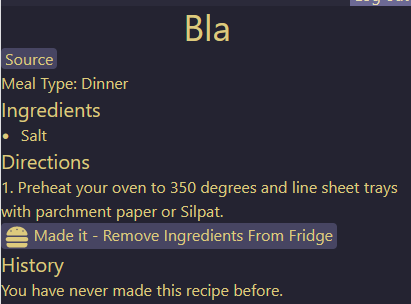
\includegraphics[scale=0.75]{figures/bad_recipe_entry.png}
\end{figure}

A possible solution for this issue would have been to further pre-process the data beyond what is
discussed in Section~\ref{sec:data_pre_process} to remove or correct noisy entries that would otherwise
harm the quality of the system.~\cite{garcia_big_2016} This was not considered a priority due to time
constraints and the fact that the noise had minimal impact on the system's results.

\subsection{Use of the Metric System (FR\arabic{metricunitsid}, FR\arabic{imperialunitsid})}

All the analysed competitors used the imperial system of measurement for their ingredients. However, this
can lead to confusion especially for users outside the US as the majority of the world uses the metric system.~\cite{pomroy_metric_2008}

For this reason, \chef{} shall use the metric system by default (FR\arabic{metricunitsid}). However, an option to
instead use the imperial system could be included for users more comfortable with it (FR\arabic{imperialunitsid}).

\subsection{Ingredient Entry (FR\arabic{manualaddid}, FR\arabic{scanbarcodeid}, FR\arabic{scanreceiptid})}

Another core feature of all analysed competitors was the ability to manually add ingredients into the respective
systems. This is a key feature for the \chef{} app and is essential for the system to function as intended.

Possible extensions to this feature were identified as the ability to scan barcodes of ingredients (FR\arabic{scanbarcodeid})
and to scan a receipt from a store (FR\arabic{scanreceiptid}). These features would serve as a more convenient way to add
ingredients, especially if there are many to add at once and could be useful features for the \chef{} app.

\subsection{Recipe Suggestion (FR\arabic{suggestionid}, FR\arabic{overloadid}, FR\arabic{trackamountsid})}
The app shall suggest recipes based on the user's available ingredients, as was a key feature in
all the analysed competitors. In addition, it shall track the amount of each ingredient the user has
as this was a feature identified to be missing from the competitors, but potentially useful for the user.

Section~\ref{sec:choice_overload} of the literature review identified the potential for choice overload,
as well as a method to reduce it. This could be implemented in the \chef{} app to improve user satisfaction.

Currently, the app shows all suggestions at once, but with further development, this could be
reduced to a more limited subset of the suggestions, with the option to view more if desired and is
discussed in further detail in Section~\ref{sec:choice_overload}.

\subsection{Recipe Similarity Algorithms (FR\arabic{findsimilarid})}\label{sec:recipe_similarity}

Recipe similarity shall be evaluated using recipe names as discussed in Section~\ref{sec:recipe_name_suggestions}
with embeddings generated by the pre-trained Universal Sentence Encoder.~\cite{cer_universal_2018} model.
This model can run in a Node.js environment via TensorFlow.js, and returns a 512-dimensional vector
for each input sentence that can then be compared using cosine similarity as used in the original
USE paper. This metric returns a normalized score between 0 and 1 for each pair of embeddings, with
higher scores indicating greater similarity. Overall, the metric provides higher precision and recall
than other metrics, making it an effective measure for ranked retrieval from queries.~\cite{ihajeer_comparison_2012}
